\documentclass[12pt,a4paper,twoside]{report}

% ------------------------------
% Core Packages
% ------------------------------
\usepackage[utf8]{inputenc}
\usepackage[T1]{fontenc}
\usepackage{lmodern}
\usepackage{microtype}
\usepackage{amsmath,amssymb,amsfonts}
\usepackage{geometry}
\usepackage{fancyhdr}
\usepackage{titlesec}
\usepackage{tocloft}
\usepackage{tocbibind}
\usepackage{graphicx}
\usepackage{float}
\usepackage{booktabs}
\usepackage{tabularray}
\usepackage{enumitem}
\usepackage{multirow}
\usepackage{multicol}
\usepackage{listings}
\usepackage{minted}
\usepackage{xcolor}
\usepackage{hyperref}
\usepackage{url}
\usepackage{datetime2}
\usepackage{tikz}
\usepackage{tikz-qtree}
\usetikzlibrary{shapes.geometric,arrows.meta,positioning,calc}

% ------------------------------
% Geometry & Layout
% ------------------------------
\geometry{
    a4paper,
    left=30mm,
    right=25mm,
    top=25mm,
    bottom=25mm,
    headheight=14pt
}

% ------------------------------
% Fancy Headers & Footers
% ------------------------------
\pagestyle{fancy}
\fancyhf{}
\fancyhead[LE,RO]{\thepage}
\fancyhead[RE]{\leftmark}
\fancyhead[LO]{\rightmark}
\renewcommand{\headrulewidth}{0.4pt}
\renewcommand{\footrulewidth}{0pt}

% ------------------------------
% Title Formatting
% ------------------------------
\titleformat{\chapter}[display]
    {\normalfont\huge\bfseries}{\chaptertitlename\ \thechapter}{20pt}{\Huge}
\titleformat{\section}
    {\normalfont\Large\bfseries}{\thesection}{1em}{}
\titleformat{\subsection}
    {\normalfont\large\bfseries}{\thesubsection}{1em}{}
\titleformat{\subsubsection}
    {\normalfont\normalsize\bfseries}{\thesubsubsection}{1em}{}

% ------------------------------
% Hyperref Setup
% ------------------------------
\hypersetup{
    colorlinks=true,
    linkcolor=blue!70!black,
    urlcolor=blue!70!black,
    citecolor=blue!70!black,
    pdfauthor={MCIPS Competition Team},
    pdftitle={MCIPS SecureLens - Full Technical Report},
    pdfsubject={Security Operations Prototype},
    pdfkeywords={cyber security, SIEM, incident response, Morocco, competition}
}

% ------------------------------
% Listings & Code
% ------------------------------
\definecolor{codebg}{rgb}{0.95,0.95,0.95}
\definecolor{comment}{rgb}{0.25,0.5,0.35}
\definecolor{keyword}{rgb}{0.6,0.15,0.15}
\definecolor{string}{rgb}{0.5,0.25,0.25}

\lstset{
    backgroundcolor=\color{codebg},
    basicstyle=\ttfamily\small,
    breaklines=true,
    commentstyle=\color{comment},
    keywordstyle=\color{keyword},
    stringstyle=\color{string},
    numbers=left,
    numberstyle=\tiny\color{gray},
    stepnumber=1,
    numbersep=8pt,
    frame=single,
    rulecolor=\color{black!30},
    captionpos=b,
    escapeinside={/*@}{@*/}
}

% ------------------------------
% List of Abbreviations
% ------------------------------
\usepackage{nomencl}
\makenomenclature
\renewcommand{\nomname}{List of Abbreviations}

% ------------------------------
% Document Start
% ------------------------------
\begin{document}

% ------------------------------
% Title Page
% ------------------------------
\begin{titlepage}
    \centering
    \vspace*{2cm}
    {\Huge \bfseries MCIPS SecureLens}\\[0.5cm]
    {\Large \itshape End-to-End Privacy-First Security Operations Prototype}\\[1.5cm]
    
    \includegraphics[width=0.6\textwidth]{docs/securelens-placeholder.png}\\[1.5cm] % Use a shield logo if you have one, or just leave as placeholder
    
    {\Large \bfseries Full Technical Report for Competition Judges}\\[1cm]
    {\large Prepared by: MCIPS Competition Team}\\[0.5cm]
    {\large Date: \today}\\[2cm]
    
    \vfill
    \begin{minipage}{0.8\textwidth}
        \centering
        \textit{This report details the architecture, security controls, evaluation, and operation of the MCIPS SecureLens prototype.}
    \end{minipage}
\end{titlepage}

% ------------------------------
% Abstract
% ------------------------------
\begin{abstract}
    \thispagestyle{empty}
    MCIPS SecureLens is a privacy-first, human-centric security operations (SecOps) prototype designed for small and midsize organizations operating in the Moroccan context. It demonstrates a complete end-to-end workflow: signal collection via an authenticated Go agent, strict privacy sanitization before any processing, explainable rules + TF-IDF threat classification, intelligent cross-signal incident correlation, explicit operator approval for sensitive actions, and verifiable execution receipts.
    
    This report provides a deep technical dive into all aspects of the system, from its architecture and trust boundaries to its AI evaluation methodology, threat model, and deployment considerations. The prototype emphasizes honesty and reproducibility, clearly distinguishing between real, production-ready components and simulated response actions.
\end{abstract}
\clearpage

% ------------------------------
% Table of Contents & Lists
% ------------------------------
\tableofcontents
\clearpage
\listoffigures
\listoftables
\printnomenclature
\clearpage

% ------------------------------
% List of Abbreviations
% ------------------------------
\nomenclature{MCIPS}{Moroccan Cyber Incident Protection System}
\nomenclature{SIEM}{Security Information and Event Management}
\nomenclature{SecOps}{Security Operations}
\nomenclature{JWT}{JSON Web Token}
\nomenclature{API}{Application Programming Interface}
\nomenclature{HMAC}{Hash-Based Message Authentication Code}
\nomenclature{TF-IDF}{Term Frequency-Inverse Document Frequency}
\nomenclature{AI}{Artificial Intelligence}
\nomenclature{ML}{Machine Learning}
\nomenclature{OIDC}{OpenID Connect}
\nomenclature{MFA}{Multi-Factor Authentication}
\nomenclature{DoS}{Denial of Service}
\nomenclature{DLP}{Data Loss Prevention}
\nomenclature{STRIDE}{Spoofing, Tampering, Repudiation, Information Disclosure, Denial of Service, Elevation of Privilege}
\nomenclature{IBAN}{International Bank Account Number}
\nomenclature{RIB}{Relevé d'Identité Bancaire}

% ------------------------------
% Chapter 1: Executive Summary & Product Brief
% ------------------------------
\chapter{Executive Summary and Product Brief}
\label{chap:summary}

\section{Overview}
MCIPS SecureLens is an honest, competition-ready prototype that prioritizes privacy, transparency, and human control over flashy claims of production-grade AI accuracy. It demonstrates a complete, end-to-end SecOps pipeline tailored to the Moroccan environment, with specific support for Moroccan IBAN/RIB, identity numbers, and phone formats in its privacy sanitizer.

\section{Key Strengths}
\begin{itemize}[label=$\checkmark$, leftmargin=*]
    \item \textbf{Privacy-First Design}: All sensitive data is normalized, obfuscated, and masked \textit{before} it touches persistence or AI services.
    \item \textbf{Explainable AI}: A rules + TF-IDF hybrid classifier with explicit component scores and decision sources.
    \item \textbf{Human-in-the-Loop}: Sensitive actions (e.g., password reset) require explicit operator approval.
    \item \textbf{Tenant Isolation}: Every data model, API endpoint, and Socket.IO room is strictly tenant-bound.
    \item \textbf{Honest Evaluation}: A reproducible 5-fold stratified out-of-fold evaluation on a curated 34-message corpus, with clear limitations stated upfront.
    \item \textbf{Auditable Workflow}: Complete audit trails, execution receipts, and timeline citations for every action and event.
\end{itemize}

\section{What is Real}
The following components are fully implemented and ready for production use (with appropriate scaling and hardening):
\begin{itemize}[noitemsep]
    \item Go agent for SMS and auth log file collection
    \item Express.js backend with REST APIs and Socket.IO
    \item FastAPI AI service with rules + TF-IDF classification
    \item Next.js frontend with mission control UI
    \item MongoDB persistence with proper tenant isolation
    \item HMAC-hashed collector credentials and JWT authentication
    \item Complete privacy sanitizer with red-team corpus testing
    \item Correlation engine with time window matching
    \item Incident service with audit trails and evidence management
    \item Statistics and timeline aggregation
    \item Copilot service with evidence-backed fallback answers
\end{itemize}

\section{What is Simulated}
The following actions are simulated (they write artifacts and receipts, but are not connected to external providers yet):
\begin{itemize}[noitemsep]
    \item Password reset/invalidation
    \item Domain/firewall blocking
    \item Local blocklist updates
\end{itemize}
These simulated components still demonstrate the full workflow, including approval, dispatching, and receipt generation.

\clearpage

% ------------------------------
% Chapter 2: System Architecture
% ------------------------------
\chapter{System Architecture}
\label{chap:architecture}

\section{Overall Architecture}
The system is composed of five core microservices plus a database, all containerized with Docker Compose for easy deployment. Figure~\ref{fig:arch} shows the high-level architecture and data flow.

\begin{figure}[h!]
    \centering
    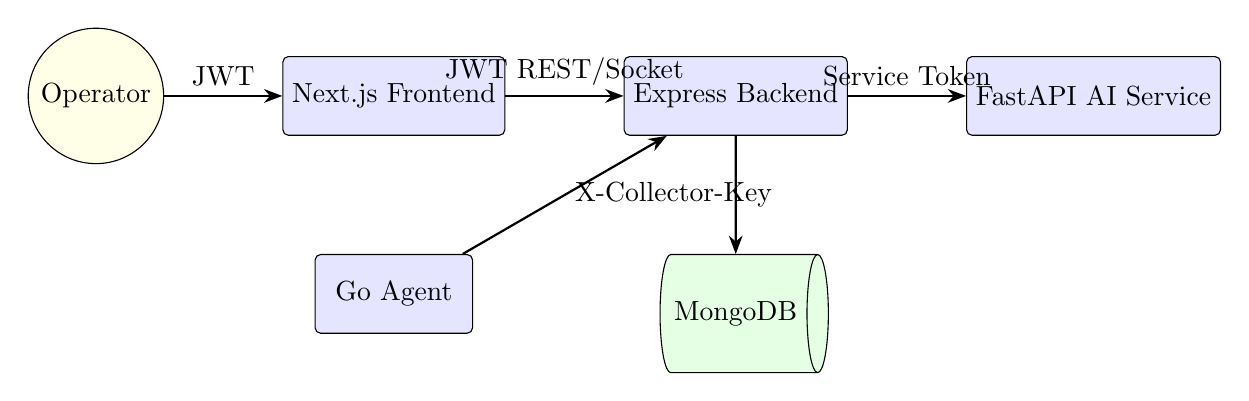
\begin{tikzpicture}[
        node distance=1.5cm and 1.5cm,
        component/.style={draw, rectangle, minimum width=2cm, minimum height=1cm, rounded corners=2pt, fill=blue!10},
        database/.style={draw, cylinder, shape aspect=0.5, minimum width=1.5cm, minimum height=1.5cm, fill=green!10},
        user/.style={draw, circle, minimum size=1.2cm, fill=yellow!10},
        arrow/.style={-Stealth, thick}
    ]
        \node[user] (operator) {Operator};
        \node[component, right=of operator] (frontend) {Next.js Frontend};
        \node[component, right=of frontend] (backend) {Express Backend};
        \node[component, right=of backend] (ai) {FastAPI AI Service};
        \node[database, below=of backend] (mongo) {MongoDB};
        \node[component, below=of frontend] (agent) {Go Agent};
        
        \draw[arrow] (operator) -- node[above] {JWT} (frontend);
        \draw[arrow] (frontend) -- node[above] {JWT REST/Socket} (backend);
        \draw[arrow] (backend) -- node[above] {Service Token} (ai);
        \draw[arrow] (backend) -- (mongo);
        \draw[arrow] (agent) -- node[right] {X-Collector-Key} (backend);
    \end{tikzpicture}
    \caption{High-level system architecture}
    \label{fig:arch}
\end{figure}

\section{Directory Structure}
The repository is organized as follows:
\begin{verbatim}
MCIPS/
├── .github/
│   └── workflows/
│       └── ci.yml          # Full CI/CD pipeline
├── agent/                  # Go signal collector
│   ├── examples/           # Sample log files
│   ├── main.go             # Agent entrypoint
│   └── main_test.go
├── ai-service/             # Python FastAPI AI service
│   ├── model-artifacts/    # TF-IDF model
│   ├── reports/            # Evaluation artifacts
│   └── src/
├── backend/                # TypeScript Express backend
│   ├── src/
│   │   ├── modules/        # Domain modules (auth, alerts, incidents, etc.)
│   │   ├── shared/         # Shared config, utils, sockets
│   │   ├── services/       # Cross-module services (correlation, etc.)
│   │   ├── tests/
│   │   └── validators/
│   └── package.json
├── docs/                   # Competition documentation
├── frontend/               # TypeScript Next.js UI
│   └── src/
├── docker-compose.yml      # Production-ready compose
└── compose.env.example     # Env file template
\end{verbatim}

\section{Trust Boundaries}
\label{sec:trust}
Trust boundaries are strictly enforced at every layer of the system:
\begin{enumerate}[label=(\alph*)]
    \item \textbf{Browser $\to$ Frontend}: Standard HTTPS (in production)
    \item \textbf{Frontend $\to$ Backend}: Bearer JWT required after login; JWT contains \texttt{tenantId} and \texttt{role}
    \item \textbf{Agent $\to$ Backend}: \texttt{X-Collector-Key} only; backend \textit{derives} tenant, adapter, source family, and event hash server-side
    \item \textbf{Backend $\to$ AI Service}: Shared service token when configured
    \item \textbf{Backend $\to$ Agent Action API}: Bearer agent token
    \item \textbf{Socket.IO}: \texttt{handshake.auth.token} required; only emits to \texttt{tenant:<tenantId>} rooms
    \item \textbf{Persistence}: MongoDB is used by default; memory mode is strictly development/test-only
\end{enumerate}

\clearpage

% ------------------------------
% Chapter 3: Threat Model
% ------------------------------
\chapter{Threat Model (STRIDE)}
\label{chap:threatmodel}

This section follows the STRIDE threat modeling methodology to document key risks, current controls, and remaining gaps.

\begin{longtblr}[
    caption={STRIDE Threat Model and Controls},
    label={tab:stride}
]{
    colspec={|X[1,l]|X[2,l]|X[3,l]|X[2,l]|},
    row{1}={font=\bfseries, bg=gray!10},
    rowhead=1
}
\hline
\textbf{Category} & \textbf{Key Risk} & \textbf{Current Control} & \textbf{Remaining Gap} \\
\hline
\textbf{Spoofing}
& Collector Impersonation
& HMAC-hashed collector keys; \texttt{X-Collector-Key} header; scopes; tenant binding; bootstrap key
& No key rotation UI yet
\\
\hline
\textbf{Spoofing}
& Socket Tenant Snooping
& Socket JWT authentication; tenant-isolated rooms; no cross-tenant event emissions
& No full OIDC/MFA user administration; single admin only
\\
\hline
\textbf{Tampering}
& Client-Supplied Tenant/Source Metadata
& Backend derives tenant, adapter, source family, and event hash server-side; client metadata ignored
& No signed provenance for collector adapters
\\
\hline
\textbf{Repudiation}
& Response Action Ambiguity
& Complete audit trail; execution receipts with provider, outcome, idempotency ID, timestamp, and artifact paths
& No external provider receipts (e.g., real AD or firewall logs)
\\
\hline
\textbf{Information Disclosure}
& Sensitive Message/PII Leakage
& Privacy sanitizer masks JWTs, API keys, IBAN/RIB, IPv6, URLs, phone numbers, and identity numbers; red-team corpus tested
& Regex masking is not a formal DLP guarantee
\\
\hline
\textbf{Denial of Service}
& Large Requests or Batches
& 256 KB request body limit; 10,000 character natural language limit; max 50 events per batch; metadata limits
& No distributed rate-limit store (uses in-memory only)
\\
\hline
\textbf{Elevation of Privilege}
& Default Secrets in Production
& Production startup rejects missing/short/known-default secrets and memory-only persistence
& No MFA; single admin only
\\
\hline
\end{longtblr}

\clearpage

% ------------------------------
% Chapter 4: Privacy Protection
% ------------------------------
\chapter{Privacy Protection}
\label{chap:privacy}

\section{Sanitizer Design}
The privacy sanitizer runs \textit{first}, before any other processing or persistence. Its design is defensive:
\begin{enumerate}
    \item \textbf{Normalize}: Normalize Unicode using NFKC and remove zero-width/bidirectional obfuscation characters
    \item \textbf{Extract}: Extract privacy-safe indicators (sender, domain hashes, bank names)
    \item \textbf{Mask}: Replace sensitive PII with placeholders (\texttt{[JWT]}, \texttt{[IBAN]}, \texttt{[PHONE]}, etc.)
\end{enumerate}

\section{Red-Team Corpus}
A dedicated red-team corpus tests 8 categories of sensitive data leakage:
\begin{itemize}[noitemsep]
    \item JWT tokens
    \item API keys
    \item Moroccan IBAN and RIB
    \item IPv6 addresses
    \item Defanged URLs
    \item Moroccan phone numbers
    \item Moroccan identity numbers
\end{itemize}

\begin{table}[h!]
    \centering
    \caption{Privacy Leakage Test Results}
    \label{tab:leakage}
    \begin{tabular}{lcr}
        \toprule
        \textbf{Category} & \textbf{Tested} & \textbf{Leaked} \\
        \midrule
        jwt & 1 & 0 \\
        api\_key & 1 & 0 \\
        moroccan\_iban & 1 & 0 \\
        rib & 1 & 0 \\
        ipv6 & 1 & 0 \\
        defanged\_url & 1 & 0 \\
        moroccan\_phone & 1 & 0 \\
        moroccan\_identity & 1 & 0 \\
        \bottomrule
        \textbf{Total} & \textbf{8} & \textbf{0} \\
    \end{tabular}
\end{table}

All tests pass: \textbf{0 categories show any leakage}.

\section{Sanitizer Code Snippet}
Here is a simplified excerpt from the privacy sanitizer's mask rule application:
\begin{lstlisting}[language=TypeScript, caption=Simplified Sanitizer Mask Rules]
const maskRule = (value: string, pattern: RegExp, replacement: string) =>
    value.replace(pattern, replacement);

const sanitizeText = (
    rawContent: string,
    opts?: { maskIp?: boolean; maskSessionId?: boolean }
) => {
    let sanitized = normalizeObfuscatedText(rawContent);
    let piiDetected = false;
    let detectedBank: string | undefined;

    // Mask Moroccan bank patterns first
    bankPatterns.forEach(pattern => {
        const match = sanitized.match(pattern);
        if (match && !detectedBank) {
            detectedBank = match[0];
            piiDetected = true;
            sanitized = maskRule(sanitized, pattern, '[BANK]');
        }
    });

    // Mask common PII
    applyMask(sanitized, emailPattern, '[EMAIL]');
    applyMask(sanitized, jwtPattern, '[JWT]');
    applyMask(sanitized, apiKeyPattern, '[API_KEY]');
    applyMask(sanitized, moroccanIbanPattern, '[IBAN]');
    applyMask(sanitized, ribPattern, '[RIB]');
    applyMask(sanitized, moroccanPhonePattern, '[PHONE]');
    applyMask(sanitized, ipv6Pattern, '[IPV6]');

    return { sanitizedContent: sanitized, piiDetected, detectedBank };
};
\end{lstlisting}

\clearpage

% ------------------------------
% Chapter 5: Threat Classification
% ------------------------------
\chapter{Threat Classification}
\label{chap:classification}

\section{Hybrid Classifier Design}
The live classifier uses a deterministic, explainable \textbf{rules + TF-IDF hybrid}:
\begin{enumerate}
    \item \textbf{Rules Engine}: First, a high-precision rules engine runs, looking for:
    \begin{itemize}[noitemsep]
        \item Morocco-relevant bank impersonation
        \item Suspicious URL patterns
        \item OTP or pressure language
        \item Login attempts from unfamiliar devices/IPs
    \end{itemize}
    \item \textbf{TF-IDF Model}: A lightweight Logistic Regression model trained on a 34-message multilingual corpus
    \item \textbf{Combination}: The hybrid uses a weighted combination, prioritizing rules to minimize false positives
\end{enumerate}

\section{Training and Evaluation}
The evaluation is a reproducible 5-fold stratified out-of-fold (OOF) design:
\begin{itemize}[noitemsep]
    \item \textbf{Dataset Size}: 34 curated messages
    \item \textbf{Labels}: 17 phishing, 17 safe
    \item \textbf{Languages}: 8 Arabic, 6 Darija, 12 English, 8 French
    \item \textbf{Final Artifact}: Trained on all 34 messages
\end{itemize}

\begin{table}[h!]
    \centering
    \caption{Classifier Performance Comparison}
    \label{tab:classifier}
    \begin{tabularx}{\textwidth}{lcccccccc}
        \toprule
        \textbf{System} & \textbf{Accuracy} & \textbf{Precision} & \textbf{Recall} & \textbf{F1} & \textbf{PR-AUC} & \textbf{ROC-AUC} & \textbf{Median (ms)} & \textbf{p95 (ms)} \\
        \midrule
        Rules & 0.6471 & 1.0000 & 0.2941 & 0.4545 & 0.7274 & 0.7145 & 0.0167 & 0.0242 \\
        ML & 0.6176 & 0.6250 & 0.5882 & 0.6061 & 0.5742 & 0.5398 & 0.2723 & 0.3736 \\
        Hybrid & 0.6471 & 1.0000 & 0.2941 & 0.4545 & 0.7475 & 0.7301 & 0.2891 & 0.4196 \\
        \bottomrule
    \end{tabularx}
\end{table}

The hybrid maintains the rules' perfect precision (no false positives), which is critical for a system that alerts operators, while slightly improving the AUC metrics.

\section{Important Limitations}
\textit{This is a pilot evaluation on a tiny, curated dataset. It demonstrates reproducibility, not production readiness.}
\begin{itemize}[noitemsep]
    \item Only 34 messages were evaluated
    \item Examples are synthetic or manually curated
    \item Per-language sample counts are too small for language-specific claims
    \item The artifact must not be the sole security control
\end{itemize}

\clearpage

% ------------------------------
% Chapter 6: Incident Workflow & Correlation
% ------------------------------
\chapter{Incident Workflow and Correlation}
\label{chap:incidents}

\section{Correlation Engine}
The correlation engine groups signals into incidents based on:
\begin{itemize}[noitemsep]
    \item \textbf{Tenant Isolation}: Strictly per-tenant
    \item \textbf{Time Window}: 20 minutes by default
    \item \textbf{Signal Types}: Phishing messages followed by login attempts are prioritized
    \item \textbf{Canonical IDs}: Reuses existing incident IDs to avoid fragmentation
\end{itemize}

\section{Incident Timeline and Evidence}
Every incident maintains:
\begin{itemize}[noitemsep]
    \item \textbf{Timeline}: Chronological list of events with stable citations (\texttt{T1}, \texttt{T2}, etc.)
    \item \textbf{Evidence}: Structured evidence records with citations (\texttt{E1}, \texttt{E2}, etc.)
    \item \textbf{MITRE ATT\&CK}: Candidate mappings with confidence scores, evidence IDs, and official URLs
    \item \textbf{Audit Trail}: Complete log of all status changes and actions
    \item \textbf{Correlated Signals}: List of all signals linked to the incident
\end{itemize}

\section{Response Actions}
Response actions have well-defined states:
\begin{enumerate}[label=\texttt{\textcolor{blue}{\arabic*}}, leftmargin=*]
    \item \texttt{pending}: Awaiting operator approval or automated execution
    \item \texttt{approved}: Operator has given consent
    \item \texttt{dispatching}: Sending to agent for execution
    \item \texttt{completed}/\texttt{failed}/\texttt{simulated}: Execution outcome
    \item \texttt{rejected}: Operator has rejected the action
\end{enumerate}

Sensitive actions (like password reset) always require explicit approval. All actions produce execution receipts.

\clearpage

% ------------------------------
% Chapter 7: Deployment & Operations
% ------------------------------
\chapter{Deployment and Operations}
\label{chap:deployment}

\section{Docker Compose}
The system comes with a production-ready \texttt{docker-compose.yml} that includes:
\begin{itemize}[noitemsep]
    \item MongoDB 7 with persistent volumes and health checks
    \item AI Service with health checks
    \item Backend with health checks and internal networking
    \item Agent with health checks and persistent runtime volume
    \item Frontend with health checks and public port mapping
\end{itemize}

\section{Required Environment Variables}
Docker Compose requires explicit secrets (see \texttt{compose.env.example}). The following are required for production:
\begin{itemize}[noitemsep]
    \item \texttt{JWT\_SECRET} (32+ characters, no defaults)
    \item \texttt{AI\_SERVICE\_TOKEN} (32+ characters)
    \item \texttt{AGENT\_API\_TOKEN} (32+ characters)
    \item \texttt{COLLECTOR\_KEY\_PEPPER} (32+ characters, for HMAC)
    \item \texttt{BOOTSTRAP\_COLLECTOR\_KEY} (32+ characters)
    \item \texttt{ADMIN\_PASSWORD\_HASH} (bcrypt hash, no default)
\end{itemize}

The backend will \textit{refuse to start} in production if any of these are missing, too short, or use known defaults.

\section{CI/CD Pipeline}
The GitHub Actions pipeline (\texttt{.github/workflows/ci.yml}) runs on every push:
\begin{enumerate}[noitemsep]
    \item Backend: Test, build, npm audit
    \item AI Service: Test, evaluate models, pip audit
    \item Frontend: Build, Playwright E2E tests, npm audit
    \item Agent: Go test, vet, build, govulncheck
    \item Docker: Full compose build
    \item Secrets: Gitleaks scan
\end{enumerate}

\clearpage

% ------------------------------
% Chapter 8: Judge Instructions & Demo Script
% ------------------------------
\chapter{Judge Instructions and 3-Minute Demo Script}
\label{chap:demo}

Full instructions are in \texttt{docs/JUDGE\_README.md} and \texttt{docs/DEMO\_SCRIPT\_3\_MIN.md}.

\section{Quick Demo Steps}
\begin{enumerate}
    \item Start the system with \texttt{docker compose up --build}
    \item Navigate to \texttt{http://localhost:3000} and login with \texttt{admin@mcips.local} / \texttt{password}
    \item Go to \textbf{Demo Lab}
    \item Click \textbf{Run Scenario} for the phishing-login example
    \item Watch the live updates flow into \textbf{Mission Control}
    \item Navigate to \textbf{Incidents}, select the new incident
    \item Go to the \textbf{Action Dock} and \textbf{Approve} the password reset action
    \item Verify the status changes from \texttt{pending} $\to$ \texttt{dispatching} $\to$ \texttt{simulated} and a receipt is shown
\end{enumerate}

\clearpage

% ------------------------------
% Appendices
% ------------------------------
\appendix

\chapter{Quick Start Guide}
\label{app:quickstart}
\section{Local Development}
\begin{enumerate}[noitemsep]
    \item Copy \texttt{compose.env.example} to \texttt{.env} and fill in secrets
    \item Run \texttt{docker compose up --build}
    \item Access the UI at \texttt{http://localhost:3000}
\end{enumerate}

\chapter{Environment File Template}
\label{app:env}
Full example in \texttt{compose.env.example}.

\chapter{Full List of Endpoints}
\label{app:api}
See \texttt{backend/src/modules/*/presentation/routes/} for full details. Key endpoints include:
\begin{itemize}[noitemsep]
    \item \texttt{POST /api/auth/login}: User login
    \item \texttt{GET /api/auth/me}: Get current user
    \item \texttt{GET /api/alerts/}: Paginated alerts
    \item \texttt{GET /api/incidents/}: Paginated incidents
    \item \texttt{PATCH /api/incidents/:id/status}: Update incident status
    \item \texttt{POST /api/incidents/:id/actions/:actionId/approve}: Approve action
    \item \texttt{POST /api/events/}: Ingest event
    \item \texttt{GET /api/stats/summary}: Get stats
    \item \texttt{POST /api/copilot/query}: Ask copilot
    \item \texttt{POST /api/simulation/once}: Run one simulation event
\end{itemize}

\chapter{Competition Documentation}
\label{app:docs}
All remaining Markdown files in \texttt{docs/} and \texttt{ai-service/reports/} are for judges:
\begin{itemize}[noitemsep]
    \item \texttt{docs/JUDGE\_README.md}: Detailed judge instructions
    \item \texttt{docs/DEMO\_SCRIPT\_3\_MIN.md}: Full 3-minute demo walkthrough
    \item \texttt{docs/REAL\_VS\_SIMULATED.md}: Exact list of real vs simulated features
    \item \texttt{ai-service/reports/evaluation\_report.md}: Full AI evaluation report
    \item \texttt{ai-service/reports/phishing\_model\_card.md}: Model card
    \item \texttt{ai-service/reports/phishing\_dataset\_card.md}: Dataset card
\end{itemize}

\clearpage

% ------------------------------
% Final Backmatter
% ------------------------------
\phantomsection
\addcontentsline{toc}{chapter}{Bibliography} % Optional, if you add a bibliography
%\bibliographystyle{plain}
%\bibliography{references}

\end{document}
